\documentclass{beamer}

%\usetheme{CambridgeUS}         % tema
% \usecolortheme{orchid}      % cores
\usetheme{metropolis}
\metroset{numbering=fraction, sectionpage=none, subsectionpage=progressbar}
\usecolortheme{seahorse}
\usecolortheme{rose}
\usefonttheme[onlysmall]{structurebold}
\usefonttheme[onlymath]{serif} % fonte modo matematico

\usepackage{framed}
\usepackage{disciplina}
\usepackage{tikz}
\usetikzlibrary{calc,shapes.multipart,chains,arrows}
\usepgflibrary{shapes.multipart}
\newcommand{\eq}{=}

\author[João Araujo Ribeiro]{João Araujo Ribeiro \\ \texttt{jaraujo@uerj.br}}
\institute[UERJ]{Universidade do Estado do Rio de Janeiro} % opcional
\date[EstrInf]{Departamento de Engenharia de Sistemas e Computação}
\pgfdeclareimage[height=0.7cm]{imagens//logo.png}{imagens//logodesc.png}
\logo{\pgfuseimage{imagens//logo.png}}
% Titulo
\title[\sc{Estruturas de Informação I}]{Estruturas de Informação I}
\subtitle{5. Tabelas de Hash}

\begin{document}

\begin{frame}
  \titlepage
\end{frame}

\begin{frame}
	\frametitle{Resumo}
	Nesta aula vamos estudar tabelas de hash.
	
	{\footnotesize \texttt{http://www.opendatastructures.org/ods-python/5\_Hash\_Tables.html}}
	\tableofcontents
\end{frame}

\section{5 - Tabelas de Hash}
\begin{frame}
	\LARGE{\alert{Tabelas de Hash}}
	
	\normalsize
	 Tabelas de Hash são métodos eficientes de armazenar um pequeno número $n$ de inteiros de uma grande faixa  $U=\{0,\ldots,2^w-1\}$. Vamos examinar os dois tipos mais comuns de implementação de tabelas de hash: Hash com encadeamento e sondagem linear
	 
	 Outros nomes possíveis são tabelas de \textbf{Dispersão} ou tabelas de \textbf{Espalhamento}.
	
\end{frame}

\begin{frame}
\frametitle{Cálculo do hash}

Frequentemente tabelas de hash armazenam dados que não são inteiros. Neste caso, o código de hash interno é calculado associando com cada item um número inteiro.	

\end{frame}

\subsection{5.1 Tabela de Dispersão por encadeamento}
\begin{frame}
\frametitle{ChainedHashTable}
Uma estrutura de tabela de dispersão por encadeamento (ChainedHashTable) utiliza a dispersão com encadeamento para armazenar dados como um array, $t$, de listas. Um inteiro, $n$, guarda o número total de itens em todas as listas.

\begin{figure}
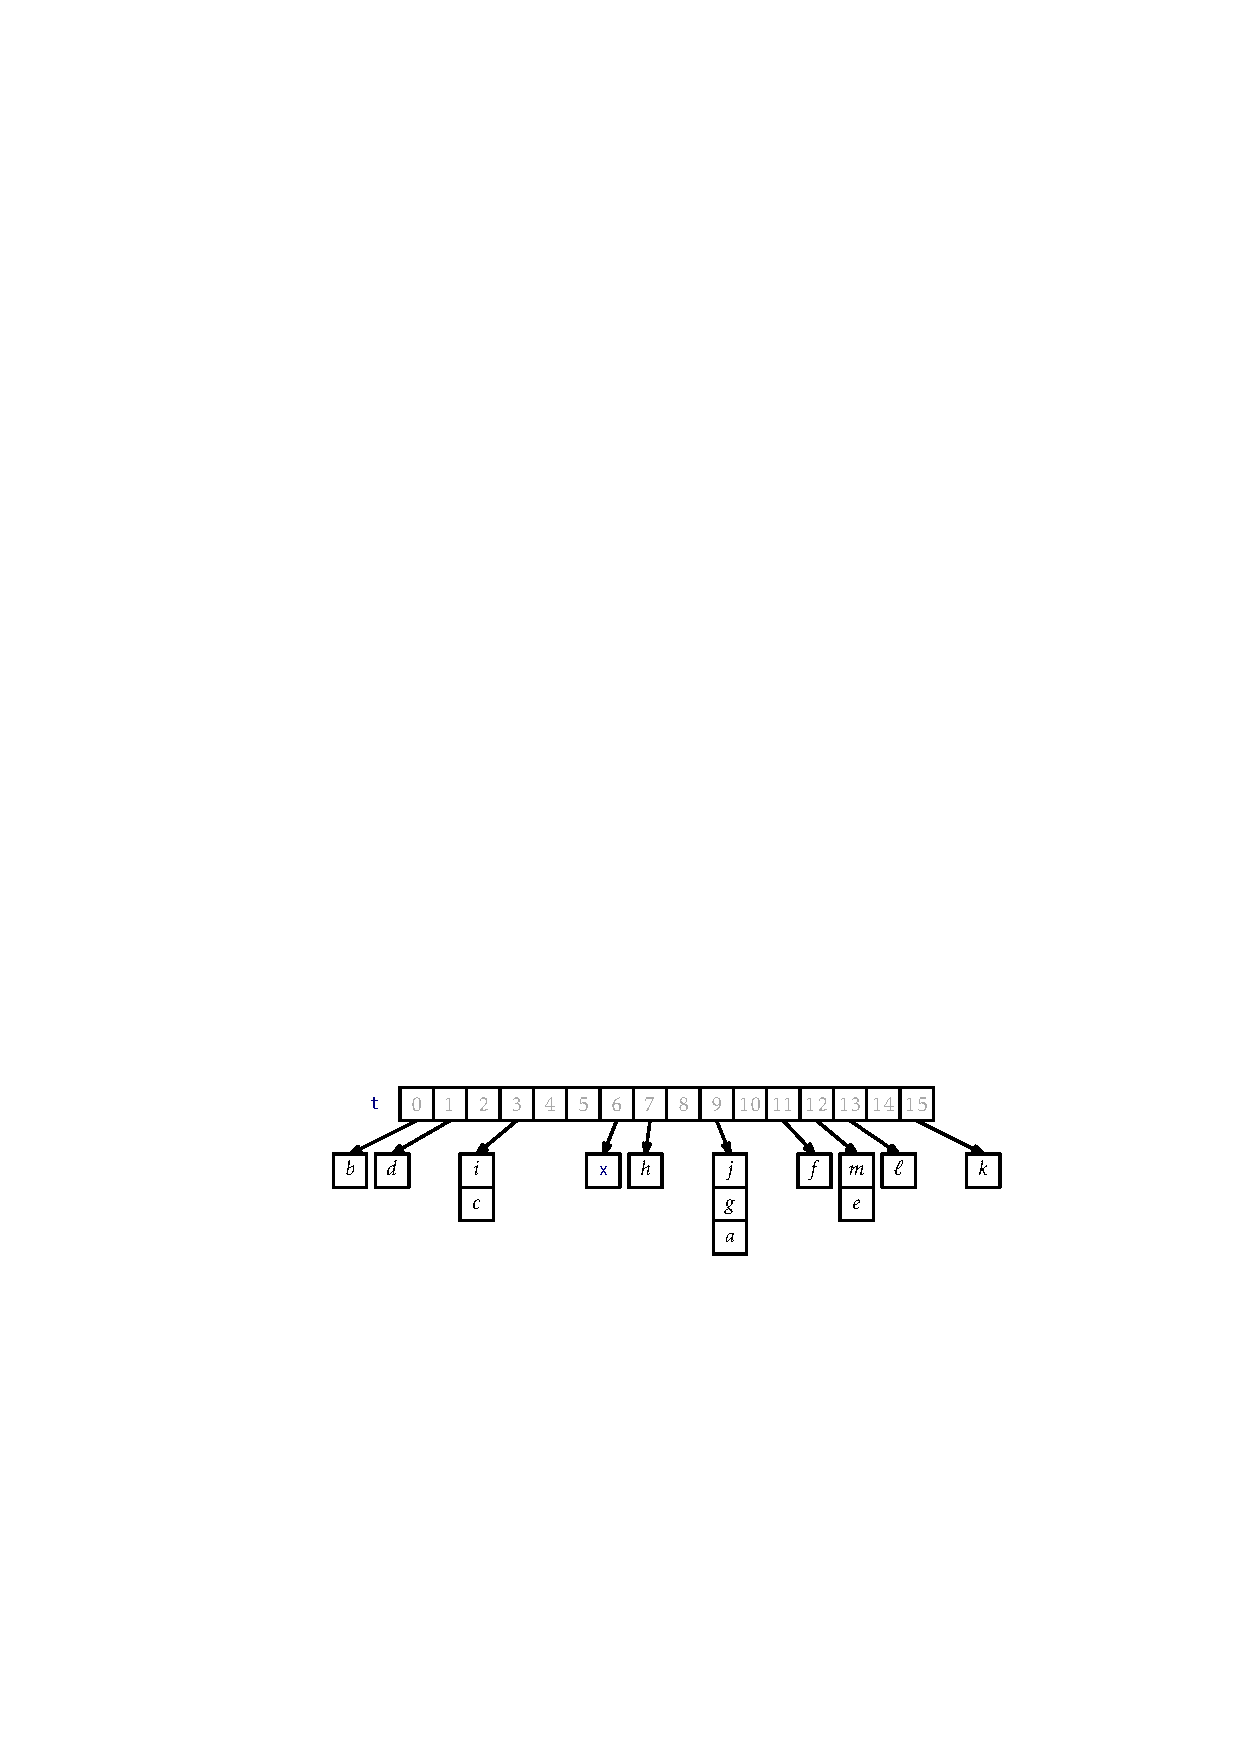
\includegraphics{imagens/chainedhashtable}
\end{figure}

\end{frame}

\begin{frame}
\frametitle{$initialize()$}
\begin{oframed}
\begin{flushleft}
\hspace*{1em} \ensuremath{\mathrm{initialize}()}\\
\hspace*{1em} \hspace*{1em} \ensuremath{d \gets  1}\\
\hspace*{1em} \hspace*{1em} \ensuremath{t \gets  \ensuremath{\mathrm{alloc\_table}(2^{d}})}\\
\hspace*{1em} \hspace*{1em} \ensuremath{z \gets  \ensuremath{\mathrm{random\_odd\_int}()}}\\
\hspace*{1em} \hspace*{1em} \ensuremath{n \gets  0}\\
\end{flushleft}
\end{oframed}

\end{frame}

\begin{frame}
\frametitle{Valor de hash}
O valor do hash de um item de dados $ \ensuremath{x}$, indicado como $ \ensuremath{\mathrm{hash}(x)}$ é um valor na faixa $ \{0,\ldots,\ensuremath{\ensuremath{\mathrm{length}(t)}}-1\}$. Todos os itens com valor de hash igual a $ \ensuremath{i}$ são armazenados na lista $ \ensuremath{t[i]}$. Para certificar-se que a lista não fique muito longa, mantemos o invariante

$\displaystyle \ensuremath{\ensuremath{n}} \le \ensuremath{\ensuremath{\mathrm{length}(t)}} $

deste modo, o número médio de elementos armazenados em uma dessas listas é $ \ensuremath{\ensuremath{n}}/\ensuremath{\ensuremath{\mathrm{length}(t)}} \le 1$. 
\end{frame}

\begin{frame}
\frametitle{$add(x$)}
Para armazenar um elemento, $ \ensuremath{x}$, na tabela de dispersão, primeiro checamos se o tamanho de $  t$ precisa ser aumentado e, se precisar, aumentamos $ t$. Com este problema resolvido, fazermos o hash $ \ensuremath{x}$ para obter um inteiro, $ \ensuremath{i}$, na faixa $ \{0,\ldots,\ensuremath{\ensuremath{\mathrm{length}(t)}}-1\}$, e acrescentamos $ \ensuremath{x}$ à lista $ \ensuremath{t[i]}$: 
\begin{oframed}
\begin{flushleft}
\hspace*{1em} \ensuremath{\mathrm{add}(x)}\\
\hspace*{1em} \hspace*{1em} {\color{black} \textbf{if}} \ensuremath{\mathrm{find}(x) \ne nil} {\color{black} \textbf{then}}  {\color{black} \textbf{return}} \ensuremath{\ensuremath{\mathit{false}}}\\
\hspace*{1em} \hspace*{1em} {\color{black} \textbf{if}} \ensuremath{n+1 > \mathrm{length}(t)} {\color{black} \textbf{then}}  \ensuremath{\mathrm{resize}()}\\
\hspace*{1em} \hspace*{1em} \ensuremath{t[\mathrm{hash}(x)].\mathrm{append}(x)}\\
\hspace*{1em} \hspace*{1em} \ensuremath{n \gets  \ensuremath{n + 1}}\\
\hspace*{1em} \hspace*{1em} {\color{black} \textbf{return}} \ensuremath{\ensuremath{\mathit{true}}}\\
\end{flushleft}
\end{oframed}

\end{frame}

\begin{frame}
\frametitle{Crescendo a tabela}
Para crescer a tabela, se necessário, envolve dobrar o tamanho de $ t$ e reinserir todos os elementos na nova tabela. Usamos a mesma estratégia da implementação da ArrayStack, com os mesmos resultados.
\end{frame}

\begin{frame}
\frametitle{$remove(x)$}
Para remover um elemento, $ \ensuremath{x}$, de uma tabela de dispersão, iteramos sobre a lista $ \ensuremath{t[\mathrm{hash}(x)]}$ até encontrar  $ \ensuremath{x}$ e então o removemos:

\begin{oframed}
\begin{flushleft}
\hspace*{1em} \ensuremath{\mathrm{remove}(x)}\\
\hspace*{1em} \hspace*{1em} \ensuremath{\ensuremath{\mathit{\ell}} \gets  \ensuremath{t[\mathrm{hash}(x)]}}\\
\hspace*{1em} \hspace*{1em} {\color{black} \textbf{for}} y {\color{black} \textbf{in}} \ensuremath{\ell} {\color{black} \textbf{do}} \\
\hspace*{1em} \hspace*{1em} \hspace*{1em} {\color{black} \textbf{if}} \ensuremath{y \eq x} {\color{black} \textbf{then}} \\
\hspace*{1em} \hspace*{1em} \hspace*{1em} \hspace*{1em} \ensuremath{\ensuremath{\mathit{\ell}}.\mathrm{remove\_value}(y)}\\
\hspace*{1em} \hspace*{1em} \hspace*{1em} \hspace*{1em} \ensuremath{n \gets  \ensuremath{n - 1}}\\
\hspace*{1em} \hspace*{1em} \hspace*{1em} \hspace*{1em} {\color{black} \textbf{if}} \ensuremath{3\cdot n < \mathrm{length}(t)} {\color{black} \textbf{then}}  \ensuremath{\mathrm{resize}()} \\
\hspace*{1em} \hspace*{1em} \hspace*{1em} \hspace*{1em} {\color{black} \textbf{return}} \ensuremath{y}\\
\hspace*{1em} \hspace*{1em} {\color{black} \textbf{return}} \ensuremath{nil} \\
\end{flushleft}
\end{oframed} 

\end{frame}

\begin{frame}
\frametitle{$find(x)$}

A busca por um elemento $ \ensuremath{x}$ em uma tabela de dispersão envolve executar uma busca linear na lista $ \ensuremath{t[\mathrm{hash}(x)]}$: 

\begin{oframed}
\begin{flushleft}
\hspace*{1em} \ensuremath{\mathrm{find}(x)}\\
\hspace*{1em} \hspace*{1em} {\color{black} \textbf{for}} y {\color{black} \textbf{in}} \ensuremath{t[\mathrm{hash}(x)]} {\color{black} \textbf{do}} \\
\hspace*{1em} \hspace*{1em} \hspace*{1em} {\color{black} \textbf{if}} \ensuremath{y \eq x} {\color{black} \textbf{then}} \\
\hspace*{1em} \hspace*{1em} \hspace*{1em} \hspace*{1em} {\color{black} \textbf{return}} \ensuremath{y}\\
\hspace*{1em} \hspace*{1em} {\color{black} \textbf{return}} \ensuremath{\ensuremath{\mathit{nil}}}\\
\end{flushleft}
\end{oframed}
\end{frame}

\begin{frame}
\frametitle{Desempenho}

O desempenho de uma tabela de dispersão depende criticamente da escolha da função de hash. Uma boa função de hash vai espalhar os elementos igualmente entre as listas $ \ensuremath{\mathrm{length}(t)}$, de modo que o tamanho esperado da lista $ \ensuremath{t[\mathrm{hash}(x)]}$ seja $ O(\ensuremath{\ensuremath{n}}/\ensuremath{\ensuremath{\mathrm{length}(t)})} = O(1)$. Por outro lado, uma função de hash mal escolhida vai posicionar todos os valores (incluindo $ \ensuremath{x}$) na mesma posição da tabela, e neste caso o tamanho da lista $ \ensuremath{t[\mathrm{hash}(x)]}$ será $n$. 

\end{frame}

\subsection{5.1.1 Hash Multiplicativo}
\begin{frame}
\frametitle{Hash Multiplicativo}
O Hash Multiplicativo é um método eficiente de gerar valores de hash baseado na aritmética modular e na divisão inteira. Ele usa o operador $ div $, que calcula a parte inteira de um quociente, descartando o resto. Formalmente, para quaisquer inteiros $ a\ge 0$ e $ b\ge 1$, $ a$ $div$ $b = \lfloor a/b\rfloor$. 
\end{frame}

\begin{frame}
\frametitle{Hash Multiplicativo}
 Em um hash multiplicativo, usamos uma tabela de dispersão de tamanho $ 2^{\ensuremath{\ensuremath{d}}}$ para algum inteiro $ \ensuremath{d}$ (chamado de dimensão). A fórmula para fazer o hash de um inteiro $ \ensuremath{\ensuremath{x}}\in\{0,\ldots,2^w-1\}$ é

\[
    \ensuremath{\ensuremath{\mathrm{hash}(x)}} = ((\ensuremath{\ensuremath{z}}\cdot\ensuremath{\ensuremath{x}}) \bmod 2^w)\, div\, 2^{\ensuremath{\ensuremath{w}}-\ensuremath{\ensuremath{d}}} \enspace.
\]


onde, $ \ensuremath{z}$ é um número aleatório ímpar em $ \{1,\ldots,2^w-1\}$. Esta função de hash pode ser implementada de modo bem eficiente se observarmos que, por default, as operações em inteiros já são feitas em módulo $2^w$ onde $\ensuremath{\ensuremath{w}}$ é o número de bits de um inteiro. 

Além disso, a divisão inteira por $ 2^{\ensuremath{\ensuremath{w}}-\ensuremath{\ensuremath{d}}}$ é equivalente a descartar os  $ \ensuremath{\ensuremath{w}}-\ensuremath{\ensuremath{d}}$ bit mais à direita em uma representação binária (que é equivalente ao deslocamento dos bits à direita por $ \ensuremath{\ensuremath{w}}-\ensuremath{\ensuremath{d}}$ usando o operador $ \ensuremath{\gg}$). 
\end{frame}

\begin{frame}
\frametitle{Função de hash}
\begin{oframed}
\begin{flushleft}
\hspace*{1em} \ensuremath{\mathrm{hash}(x)}\\
\hspace*{1em} \hspace*{1em} {\color{black} \textbf{return}} (\ensuremath{(z \cdot  \mathrm{calc\_hash}(x)) \bmod  2^{w}}) \ensuremath{\gg} \ensuremath{(w-d)}\\
\end{flushleft}
\end{oframed}
\begin{figure}
  \begin{center}
    \resizebox{.98\textwidth}{!}{
    \setlength{\arrayrulewidth}{1pt}
    \begin{tabular}{|lr@{}r|}\hline
    $2^\ensuremath{\ensuremath{w}}$ (4294967296)&            \ensuremath{1}&\ensuremath{\ensuremath{00000000000000000000000000000000}} \\
    \ensuremath{\ensuremath{z}} (4102541685)&                   &\ensuremath{\ensuremath{11110100100001111101000101110101}} \\
    \ensuremath{\ensuremath{x}} (42) &                          &\ensuremath{\ensuremath{00000000000000000000000000101010}} \\
    $\ensuremath{\ensuremath{z}}\cdot\ensuremath{\ensuremath{x}}$ &             \ensuremath{\ensuremath{101000}}&\ensuremath{\ensuremath{00011110010010000101110100110010}} \\
    $(\ensuremath{\ensuremath{z}}\cdot\ensuremath{\ensuremath{x}})\bmod 2^w$ &      &\ensuremath{\ensuremath{00011110010010000101110100110010}} \\
    $((\ensuremath{\ensuremath{z}}\cdot\ensuremath{\ensuremath{x}})\bmod 2^w)\, div \, 2^{\ensuremath{\ensuremath{w}}-\ensuremath{\ensuremath{d}}}$ &&
                      \multicolumn{1}{@{}l|}{\ensuremath{\ensuremath{00011110}}} \\\hline
    \end{tabular}}
    \setlength{\arrayrulewidth}{.4pt}
  \end{center}
  \caption{A operação de hash multiplicativo com $\ensuremath{\ensuremath{w}}=32$
    e $\ensuremath{\ensuremath{d}}=8$.}
\end{figure}

\end{frame}

\subsection{5.2 Sondagem Linear}
\begin{frame}
\frametitle{Hash Linear}
Uma alternativa para armazenar elementos, chamada de endereçamento aberto,coloca os itens diretamente em um array, $ t$, e cada posição do array armazena no máximo um valor. Em alguns lugares esta abordagem é chamada de endereçamento aberto com sondagem linear. 
\end{frame}

\begin{frame}
\frametitle{LinearHashTable}
A ideia em uma LinearHashTable é que gostaríamos de armazenar o elemento $ \ensuremath{x}$ com valor de hash $ \ensuremath{i\gets \ensuremath{\mathrm{hash}(x)}}$ na posição da tabela $ \ensuremath{t[i]}$. Se não podemos (porque algum elemento já está armazenado ali), tentamos armazená-lo na posição $t[(\ensuremath{\ensuremath{i}}+1)\bmod\ensuremath{\ensuremath{\mathrm{length}(t)}}]$;
se isto ainda não é possível, tentamos $t[(\ensuremath{\ensuremath{i}}+2)\bmod\ensuremath{\ensuremath{\mathrm{length}(t)}}]$, e assim por diante até encontrarmos um lugar para \ensuremath{\ensuremath{x}}.

\end{frame}

\begin{frame}
\frametitle{Entradas}
Existem três tipos de entradas armazenadas em t: 
\begin{enumerate}
  \item valores de dados: valores reais no USet que estamos representando;
  \item valores \ensuremath{\ensuremath{\ensuremath{\mathit{nil}}}}: nas posições do array nas quais nunca nenhum dado foi armazenado; e
  \item valores \ensuremath{\ensuremath{\ensuremath{\mathit{del}}}}: nas posições do array nas quais dados foram alguma vez armazenados mas que foram apagados.
\end{enumerate}

\end{frame}

\begin{frame}
\frametitle{Tamanho de $t$}
Além do contador, \ensuremath{\ensuremath{n}}, que acompanha o número de elementos em uma LinearHashTable, um contador, \ensuremath{\ensuremath{q}}, acompanha o número de elementos dos tipos~1 e 3.  Isto é, \ensuremath{\ensuremath{q}} é igual a  \ensuremath{\ensuremath{n}} mais o número de valores \ensuremath{\ensuremath{\ensuremath{\mathit{del}}}} em t.  Para isso funcionar de modo eficiente, precisamos que 
t seja consideravelmente maior que \ensuremath{\ensuremath{q}}, de modo a haver muitos valores \ensuremath{\ensuremath{\ensuremath{\mathit{nil}}}}
em t.  As operações em uma LinearHashTable mantém um invariante $\ensuremath{\ensuremath{\mathrm{length}(t)}}\ge 2\ensuremath{\ensuremath{q}}$.
\end{frame}

\begin{frame}
\frametitle{Invariante}
Para resumir, uma LinearHashTable contém um array, $ t$, que armazena elementos de dados, e inteiros $n$ e $ \ensuremath{q}$ que acompanham o número de elementos de dados e de elementos não $ \ensuremath{\ensuremath{\mathit{nil}}}$ de $ t$, respectivamente. Como muitas funções de hash trabalham somente com tabelas de tamanho que sejam potência de  2, também usamos um inteiro $ \ensuremath{d}$ para assegurar a invariante $ \ensuremath{\ensuremath{\mathrm{length}(t)}}=2^\ensuremath{\ensuremath{d}}$. 

\end{frame}

\begin{frame}
\frametitle{$initialize()$}
\begin{oframed}
\begin{flushleft}
\hspace*{1em} \ensuremath{\mathrm{initialize}()}\\
\hspace*{1em} \hspace*{1em} \ensuremath{\mathit{del} \gets  \ensuremath{\mathrm{object}()}}\\
\ \\
\hspace*{1em} \ensuremath{\mathrm{initialize}()}\\
\hspace*{1em} \hspace*{1em} \ensuremath{d \gets  1}\\
\hspace*{1em} \hspace*{1em} \ensuremath{t \gets  \ensuremath{\mathrm{new\_array}(2^{d}})}\\
\hspace*{1em} \hspace*{1em} \ensuremath{q \gets  0}\\
\hspace*{1em} \hspace*{1em} \ensuremath{n \gets  0}\\
\end{flushleft}
\end{oframed}

\end{frame}

\begin{frame}
\frametitle{$find()$}

Começamos na entrada do array \ensuremath{\ensuremath{t[i]}} onde $\ensuremath{\ensuremath{i}}=\ensuremath{\ensuremath{\mathrm{hash}(x)}}$ e procuramos as entradas \ensuremath{\ensuremath{t[i]}},
$t[(\ensuremath{\ensuremath{i}}+1)\bmod \ensuremath{\ensuremath{\mathrm{length}(t)}}]$, $t[(\ensuremath{\ensuremath{i}}+2)\bmod \ensuremath{\ensuremath{\mathrm{length}(t)}}]$, e assim por diante,
até encontrarmos um índice \ensuremath{i'} tal que, ou, \ensuremath{\ensuremath{t[i']\gets x}}, ou \ensuremath{\ensuremath{t[i']\gets \ensuremath{nil}}}.
No primeiro caso, retornamos \ensuremath{\ensuremath{t[i']}}. No último caso, concluímos que \ensuremath{\ensuremath{x}} não está na tabela e retornamos \ensuremath{\ensuremath{\ensuremath{\mathit{nil}}}}.
\end{frame}

\begin{frame}
	\frametitle{$find()$}
\begin{oframed}
\begin{flushleft}
\hspace*{1em} \ensuremath{\mathrm{find}(x)}\\
\hspace*{1em} \hspace*{1em} \ensuremath{i \gets  \ensuremath{\mathrm{hash}(x)}}\\
\hspace*{1em} \hspace*{1em} {\color{black} \textbf{while}} \ensuremath{t[i] \ne nil} {\color{black} \textbf{do}} \\
\hspace*{1em} \hspace*{1em} \hspace*{1em} {\color{black} \textbf{if}} \ensuremath{t[i] \ne \mathit{del}} {\color{black} \textbf{and}} \ensuremath{x \eq t[i]} {\color{black} \textbf{then}}  \\
\hspace*{1em} \hspace*{1em} \hspace*{1em} \hspace*{1em} {\color{black} \textbf{return}} \ensuremath{t[i]}\\
\hspace*{1em} \hspace*{1em} \hspace*{1em} \ensuremath{i \gets  \ensuremath{(i + 1) \bmod  \mathrm{length}(t)}}\\
\end{flushleft}
\end{oframed}

\end{frame}

\begin{frame}
\frametitle{$add(x)$}

Após checar que $ \ensuremath{x}$ não está já na tabela (usando $ \ensuremath{\mathrm{find}(x)}$), procuramos $t[(\ensuremath{\ensuremath{i}}+1)\bmod \ensuremath{\ensuremath{\mathrm{length}(t)}}]$, $t[(\ensuremath{\ensuremath{i}}+2)\bmod \ensuremath{\ensuremath{\mathrm{length}(t)}}]$,
e assim por diante, até encontrarmos um \ensuremath{\ensuremath{\ensuremath{\mathit{nil}}}} ou \ensuremath{\ensuremath{\ensuremath{\mathit{del}}}} e colocamos \ensuremath{\ensuremath{x}} nesta posição,
incrementando \ensuremath{\ensuremath{n}}, e \ensuremath{\ensuremath{q}}, se apropriado.
\end{frame} 

\begin{frame}
	\frametitle{$add(x)$}
\begin{oframed}
\begin{flushleft}
\hspace*{1em} \ensuremath{\mathrm{add}(x)}\\
\hspace*{1em} \hspace*{1em} {\color{black} \textbf{if}} \ensuremath{\mathrm{find}(x) \ne nil} {\color{black} \textbf{then}}  {\color{black} \textbf{return}} \ensuremath{\ensuremath{\mathit{false}}}\\
\hspace*{1em} \hspace*{1em} {\color{black} \textbf{if}} \ensuremath{2\cdot (q+1) > \mathrm{length}(t)} {\color{black} \textbf{then}}  \ensuremath{\mathrm{resize}()}\\
\hspace*{1em} \hspace*{1em} \ensuremath{i \gets  \ensuremath{\mathrm{hash}(x)}}\\
\hspace*{1em} \hspace*{1em} {\color{black} \textbf{while}} \ensuremath{t[i] \ne nil} {\color{black} \textbf{and}} \ensuremath{t[i] \ne \mathit{del}} {\color{black} \textbf{do}} \\
\hspace*{1em} \hspace*{1em} \hspace*{1em} \ensuremath{i \gets  \ensuremath{(i + 1) \bmod  \mathrm{length}(t)}}\\
\hspace*{1em} \hspace*{1em} {\color{black} \textbf{if}} \ensuremath{t[i] \eq nil} {\color{black} \textbf{then}}  \ensuremath{q \gets  \ensuremath{q + 1}}\\
\hspace*{1em} \hspace*{1em} \ensuremath{n \gets  \ensuremath{n + 1}}\\
\hspace*{1em} \hspace*{1em} \ensuremath{t[i] \gets  x}\\
\hspace*{1em} \hspace*{1em} {\color{black} \textbf{return}} \ensuremath{\ensuremath{\mathit{true}}}\\
\end{flushleft}
\end{oframed}

\end{frame}

\begin{frame}
\frametitle{$remove(x)$}
Procuramos \ensuremath{\ensuremath{t[i]}}, $t[(\ensuremath{\ensuremath{i}}+1)\bmod \ensuremath{\ensuremath{\mathrm{length}(t)}}]$, $t[(\ensuremath{\ensuremath{i}}+2)\bmod
\ensuremath{\ensuremath{\mathrm{length}(t)}}]$, e assim por diante até acharmos um índice \ensuremath{i'} tal que \ensuremath{\ensuremath{t[i']\gets x}}
or \ensuremath{\ensuremath{t[i']\gets \ensuremath{nil}}}.  No primeiro caso, fazemos \ensuremath{\ensuremath{t[i']\gets \ensuremath{del}}} e retornamos
\ensuremath{\ensuremath{\ensuremath{\mathit{true}}}}.  No segundo caso, conclupimos que \ensuremath{\ensuremath{x}} não está armazenado na tabela (e portanto não pode ser removido) e retornamos \ensuremath{\ensuremath{\ensuremath{\mathit{false}}}}.

\end{frame}

\begin{frame}
\frametitle{$remove(x)$}

\begin{oframed}
\begin{flushleft}
\hspace*{1em} \ensuremath{\mathrm{remove}(x)}\\
\hspace*{1em} \hspace*{1em} \ensuremath{i \gets  \ensuremath{\mathrm{hash}(x)}}\\
\hspace*{1em} \hspace*{1em} {\color{black} \textbf{while}} \ensuremath{t[i] \ne nil} {\color{black} \textbf{do}} \\
\hspace*{1em} \hspace*{1em} \hspace*{1em} \ensuremath{y \gets  \ensuremath{t[i]}}\\
\hspace*{1em} \hspace*{1em} \hspace*{1em} {\color{black} \textbf{if}} \ensuremath{y \ne \mathit{del}} {\color{black} \textbf{and}} \ensuremath{x \eq y} {\color{black} \textbf{then}} \\
\hspace*{1em} \hspace*{1em} \hspace*{1em} \hspace*{1em} \ensuremath{t[i] \gets  \ensuremath{\mathit{del}}}\\
\hspace*{1em} \hspace*{1em} \hspace*{1em} \hspace*{1em} \ensuremath{n \gets  \ensuremath{n - 1}}\\
\hspace*{1em} \hspace*{1em} \hspace*{1em} \hspace*{1em} {\color{black} \textbf{if}} \ensuremath{8\cdot n < \mathrm{length}(t)} {\color{black} \textbf{then}}  \ensuremath{\mathrm{resize}()}\\
\hspace*{1em} \hspace*{1em} \hspace*{1em} \hspace*{1em} {\color{black} \textbf{return}} \ensuremath{y}\\
\hspace*{1em} \hspace*{1em} \hspace*{1em} \ensuremath{i \gets  \ensuremath{(i + 1) \bmod  \mathrm{length}(t)}}\\
\hspace*{1em} \hspace*{1em} {\color{black} \textbf{return}} \ensuremath{\ensuremath{\mathit{nil}}}\\
\end{flushleft}
\end{oframed}

\end{frame}

\begin{frame}
\frametitle{$resize()$}
Primeiro encontramos o menor inteiro não-negativo  \ensuremath{\ensuremath{d}} tal que $2^{\ensuremath{\ensuremath{d}}}
\ge 3\ensuremath{\ensuremath{n}}$.  Realocamos um array t de modo que seu tamanho seja $2^{\ensuremath{\ensuremath{d}}}$,
e então inserimos todos os elementos da antiga versão t na cópia recém alocada de t.  Enquanto fazemos, resetamos \ensuremath{\ensuremath{q}} para  \ensuremath{\ensuremath{n}}
posto que o novo array t não contém valores \ensuremath{\ensuremath{\ensuremath{\mathit{del}}}}.

\end{frame}

\begin{frame}
\frametitle{$resize()$}
\begin{oframed}
\begin{flushleft}
\hspace*{1em} \ensuremath{\mathrm{resize}()}\\
\hspace*{1em} \hspace*{1em} \ensuremath{d \gets  1}\\
\hspace*{1em} \hspace*{1em} {\color{black} \textbf{while}} (\ensuremath{2^{d} < 3\cdot n}) {\color{black} \textbf{do}}  \ensuremath{d \gets  \ensuremath{d + 1}}\\
\hspace*{1em} \hspace*{1em} \ensuremath{\ensuremath{\mathit{told}} \gets  t}\\
\hspace*{1em} \hspace*{1em} \ensuremath{t \gets  \ensuremath{\mathrm{new\_array}(2^{d}})}\\
\hspace*{1em} \hspace*{1em} \ensuremath{q \gets  n}\\
\hspace*{1em} \hspace*{1em} {\color{black} \textbf{for}} x {\color{black} \textbf{in}} \ensuremath{told} {\color{black} \textbf{do}} \\
\hspace*{1em} \hspace*{1em} \hspace*{1em} {\color{black} \textbf{if}} \ensuremath{x \ne nil} {\color{black} \textbf{and}} \ensuremath{x \ne \mathit{del}} {\color{black} \textbf{then}} \\
\hspace*{1em} \hspace*{1em} \hspace*{1em} \hspace*{1em} \ensuremath{i \gets  \ensuremath{\mathrm{hash}(x)}}\\
\hspace*{1em} \hspace*{1em} \hspace*{1em} \hspace*{1em} {\color{black} \textbf{while}} \ensuremath{t[i] \ne nil} {\color{black} \textbf{do}}  \\
\hspace*{1em} \hspace*{1em} \hspace*{1em} \hspace*{1em} \hspace*{1em} \ensuremath{i \gets  \ensuremath{(i+1) \bmod  \mathrm{length}(t)}}\\
\hspace*{1em} \hspace*{1em} \hspace*{1em} \hspace*{1em} \ensuremath{t[i] \gets  x}\\
\end{flushleft}
\end{oframed}


\end{frame}

\subsection{5.2.3 Hash por tabulação}
\begin{frame}
\frametitle{Hash por tabulação}
Para os algoritmos funcionarem idealmente, partimos de uma pressuposição forte: de que para qualquer conjunto de elementos, $\{\ensuremath{\ensuremath{x}}_1,\ldots,\ensuremath{\ensuremath{x}}_\ensuremath{\ensuremath{n}}\}$,
os valores de hash  $\ensuremath{\ensuremath{\ensuremath{\mathit{hash}}}}($x$_1),\ldots,\ensuremath{\ensuremath{\ensuremath{\mathit{hash}}}}(\ensuremath{\ensuremath{x}}_\ensuremath{\ensuremath{n}})$ são independentes e uniformemente distribuídos sobre o conjunto $\{0,\ldots,\ensuremath{\ensuremath{\mathrm{length}(t)}}-1\}$.  Uma maneira de obter isso é alocar um array gigante, \ensuremath{\ensuremath{\ensuremath{\mathit{tab}}}}, de tamanho $2^w$,
onde cada entrada é um inteiro aleatório de \ensuremath{\ensuremath{w}}-bits, independente de todas as outras entradas.  Desta forma, podemos implementar \ensuremath{\ensuremath{\mathrm{hash}(x)}} pela extração de um inteiro de \ensuremath{\ensuremath{d}}-bits de \ensuremath{\ensuremath{\ensuremath{\mathit{tab}}[x.\mathrm{hash\_code}()]}}:
%importing \codeimport{ods/LinearHashTable.idealHash(x)}: 
\begin{oframed}
\begin{flushleft}
\hspace*{1em} \ensuremath{\mathrm{ideal\_hash}(x)}\\
\hspace*{1em} \hspace*{1em} {\color{black} \textbf{return}} \ensuremath{\ensuremath{\mathit{tab}}[x.\mathrm{hash\_code}()] \ensuremath{\gg} w-d}\\
\end{flushleft}
\end{oframed}
\end{frame}

\begin{frame}
\frametitle{Hash por tabulação}
Infelizmente, armazenar um array de tamanho $2^w$ é proibitivo em termos de uso de memória.  O enfoque usado pelo \emph{hash por tabulação} é, em vez disso, tratar o inteiro de \ensuremath{\ensuremath{w}}-bits como sendo composto de $\ensuremath{\ensuremath{w}}/\ensuremath{\ensuremath{r}}$
inteiros, cada um tendo apenas $\ensuremath{\ensuremath{r}}$ bits.  Deste modo, o hash por tabulação precisa apenas de  $\ensuremath{\ensuremath{w}}/\ensuremath{\ensuremath{r}}$ arrays, cada um com tamanho $2^{\ensuremath{\ensuremath{r}}}$.  Todas as entradas deste array são inteiros de \ensuremath{\ensuremath{w}}-bit independentes e aleatórios.  Para obter o valor de \ensuremath{\ensuremath{\mathrm{hash}(x)}} dividimos  \ensuremath{\ensuremath{x.\mathrm{hash\_code}()}} em $\ensuremath{\ensuremath{w}}/\ensuremath{\ensuremath{r}}$ inteiros de \ensuremath{\ensuremath{r}}-bits e usamos estes índices dentro desses arrays.  Então combinamos todos estes valores com um operador ou-exclusivo bit-a-bit para obter \ensuremath{\ensuremath{\mathrm{hash}(x)}}.

\end{frame}



\begin{frame}
\frametitle{$hash(x)$}
\begin{oframed}
\begin{flushleft}
\hspace*{1em} \ensuremath{\mathrm{hash}(x)}\\
\hspace*{1em} \hspace*{1em} \ensuremath{h \gets  \ensuremath{\mathrm{hash\_code}(x)}}\\
\hspace*{1em} \hspace*{1em} {\color{black} \textbf{return}}  (\ensuremath{\ensuremath{\mathit{tab}}[0]}[\ensuremath{h \wedge \mathrm{ff}_{16}}] \\\
\hspace*{1em} \hspace*{1em} \hspace*{1em} \hspace*{1em}  \ensuremath{\oplus} \ensuremath{\ensuremath{\mathit{tab}}[1]}[\ensuremath{(h\ensuremath{\gg}8) \wedge \mathrm{ff}_{16}}] \\\
\hspace*{1em} \hspace*{1em} \hspace*{1em} \hspace*{1em}  \ensuremath{\oplus} \ensuremath{\ensuremath{\mathit{tab}}[2]}[\ensuremath{(h\ensuremath{\gg}16) \wedge \mathrm{ff}_{16}}] \\\
\hspace*{1em} \hspace*{1em} \hspace*{1em} \hspace*{1em}  \ensuremath{\oplus} \ensuremath{\ensuremath{\mathit{tab}}[3]}[\ensuremath{(h\ensuremath{\gg}24) \wedge \mathrm{ff}_{16}}]) \ensuremath{\gg} \ensuremath{(w-d)}\\
\end{flushleft}
\end{oframed}
Neste caso, \ensuremath{\ensuremath{\ensuremath{\mathit{tab}}}} é um array bidimensional com quatro colunas e 
$2^{32/4}=256$ linhas.

\end{frame}

\subsection{5.3 Códigos de Hash}
\begin{frame}
\frametitle{Códigos de Hash}
As tabelas de hash discutidas até aqui são usadas para associar chaves inteiras que consistem de \ensuremath{\ensuremath{w}} bits.  Em muitos casos, temos chaves que não são inteiros.  Elas podem ser strings, objetos, arrays,
ou outra estrutura composta.  Para usar tabelas de hash para este tipo de dado,
devemos mapear esses tipos de dados para códigos de hash com \ensuremath{\ensuremath{w}}-bits.  

\end{frame}

\begin{frame}
Mapeamentos de códigos de hash devem ter as seguintes propriedades:

\begin{enumerate}
  \item Se \ensuremath{\ensuremath{x}} e \ensuremath{\ensuremath{y}} são iguais, então \ensuremath{\ensuremath{x.\mathrm{hash\_code}()}} e \ensuremath{\ensuremath{y.\mathrm{hash\_code}()}}
  são iguais.

  \item Se \ensuremath{\ensuremath{x}} e \ensuremath{\ensuremath{y}} não são iguais, então a probabilidade que
  $\ensuremath{\ensuremath{x.\mathrm{hash\_code}()}}=\ensuremath{\ensuremath{y.\mathrm{hash\_code}()}}$ deve ser pequena (próxima a
  $1/2^w$).
\end{enumerate}
\end{frame}

\begin{frame}
\frametitle{Códigos de Hash para Tipos Primitivos}
Tipos de dados menores como \ensuremath{\ensuremath{\ensuremath{\mathit{char}}}}, \ensuremath{\ensuremath{\ensuremath{\mathit{byte}}}}, \ensuremath{\ensuremath{\ensuremath{\mathit{int}}}}, e \ensuremath{\ensuremath{\ensuremath{\mathit{float}}}} geralmente são fáceis de encontrar códigos de hash para eles.  Estes tipos de dados sempre têm uma representação binária e ela geralmente consiste de
\ensuremath{\ensuremath{w}} ou menos bits. Nestes casos, apenas tratamos esses bitas como a representação de um inteiro na faixa $\{0,\ldots,2^\ensuremath{\ensuremath{w}}-1\}$.  Se dois valores são diferentes, eles vão obter códigos diferentes.  Se eles são iguais, eles obtêm o mesmo código de hash.
\end{frame}

\begin{frame}
\frametitle{Códigos de Hash para Objetos Compostos}
Para um objeto composto, queremos criar um código de hash combinando os códigos de hash individuais das partes constituintes do objeto.  Isto não é muito fácil.  Embora possa haver muitos hacks para isso (por exemplo, combinando os códigos de hash com operações bit-a-bit ou exclusivo), muitos desses hacks podem facilmente falhar.
Contudo, se queremos fazer aritmética com  $2\ensuremath{\ensuremath{w}}$ bits de precisão, então existem métodos simples e robustos disponíveis.
\end{frame}

\begin{frame}
Suponha que temos um objeto composto de diversas partes
$P_0,\ldots,P_{r-1}$ cujos códigos de hah são $\ensuremath{\ensuremath{x}}_0,\ldots,\ensuremath{\ensuremath{x}}_{r-1}$.
Então, podemos escolher inteiros aleatórios mutuamente independentes com \ensuremath{\ensuremath{w}}-bits
$\ensuremath{\ensuremath{z}}_0,\ldots,\ensuremath{\ensuremath{z}}_{r-1}$ e um inteiro ímpar e aleatório de $2\ensuremath{\ensuremath{w}}$-bits \ensuremath{\ensuremath{z}} e calculamos um código de hash com
\[
   h(\ensuremath{\ensuremath{x}}_0,\ldots,\ensuremath{\ensuremath{x}}_{r-1}) =  
   \left(\left(\ensuremath{\ensuremath{z}}\sum_{i=0}^{r-1} \ensuremath{\ensuremath{z}}_i \ensuremath{\ensuremath{x}}_i\right)\bmod 2^{2\ensuremath{\ensuremath{w}}}\right)
   \, div \, 2^w \enspace .
\]

\end{frame}

\begin{frame}[shrink]
\frametitle{{hash\_code}()}
\begin{oframed}
\begin{flushleft}
 \ensuremath{\mathrm{hash\_code}()}\\
\hspace*{1em}  \ensuremath{z \gets  [\ensuremath{\mathrm{2058cc50}_{16}, \mathrm{cb19137e}_{16}, \mathrm{2cb6b6fd}_{16}}]}\\
\hspace*{1em} \ensuremath{\ensuremath{\mathit{zz}} \gets  \ensuremath{\mathrm{bea0107e5067d19d}_{16}}}\\
 \hspace*{1em} \ensuremath{h \gets  [\ensuremath{\ensuremath{\mathit{x_0}}.\mathrm{hash\_code}(), \ensuremath{\mathit{x_1}}.\mathrm{hash\_code}(), \ensuremath{\mathit{x_2}}.\mathrm{hash\_code}()}]}\\
 \hspace*{1em} {\color{black} \textbf{return}} \ensuremath{((\ensuremath{(z[0]\cdot h[0] + z[1]\cdot h[1] + z[2]\cdot h[2])\cdot zz})\bmod \ensuremath{2^{2}\cdot w)}) \ensuremath{\gg} w}\\
\end{flushleft}
\end{oframed}

\end{frame}



\begin{frame}
FIM
\end{frame}
\end{document}
